\cleardoublepage

\chapter{Introducción}

%\label{ch:chapter1}
%\section{Introducción}
\label{makereference}
El presente documento recoge el proceso de creación de un prototipo como solución integral de domótica programable, gestionada mediante software para plataforma móvil y Web App. Se plantea además cubrir una serie de objetivos adicionales que permitirán a esta solución ahorrar costes económicos y gastos innecesarios de los suministros de luz y agua en el hogar. La naturaleza del proyecto posee una vertiente sostenible, asequible y libre. Para poder cumplir con estos objetivos, será necesario que los materiales y dispositivos utilizados para su implementación sean sencillos de adquirir, fáciles de reemplazar además de tener un bajo coste en precio de adquisición y de tiempo necesario para su instalación, todo ello usando como base software y hardware libre.

\section{Motivación}
\label{makereference1.1}

Una vivienda con inquilinos requiere de dos suministros básicos, luz y agua. Generalmente se incluye un tercero, el gas. Para este proyecto consideraremos solo los dos primeros, ya que resultan más sencillos de manipular y medir. Es más sencillo cerrar una llave de paso de agua o acceder al cableado eléctrico en los cajetines de las paredes que manipular las tuberías de gas, las cuales deben manipularse con extremo cuidado dada su naturaleza volátil. Esto no significa que no haya riesgos en la manipulación de los otros dos suministros, pero es más seguro incluir un dispositivo en la red eléctrica ya sea mediante enchufes o empalmes, o incluir a un grifo una bomba de agua que manipular una cañería de gas.

El gasto medio de un hogar en España [según fuentes* INE o bien Instituto para la Diversificación y Ahorro de la Energía (IDAE)]. Existen distintas estrategias para reducir estos costes, algunas impulsadas por iniciativas gubernamentales como la introducida por el Ministerio de Industria, Turismo y Comercio con el bono para canjear de forma gratuita una bombilla convencional por dos de bajo consumo [insertar referencia Ej: http://www.rtve.es/noticias/20090706/industria-comienza-repartir-gratis-20-millones-bombillas-bajo-consumo/283773.shtml]. Otras mediante subvenciones como las cedidas por el Ministerio de Energía, Turismo y Agenda Digital a través del IDAE[ ref Ej: http://www.idae.es/ayudas-y-financiacion/para-rehabilitacion-de-edificios-programa-pareer/programa-de-ayudas-para-la].Otras basadas en la adquisición de electrodomésticos con alta eficiencia energética y consejos de `vox populi` que orientan un uso adecuado del agua y la luz. Todas estas estrategias son adecuadas y pueden combinarse entre sí para reducir el consumo y maximizar el ahorro. De hecho, los consejos comunes que se recomiendan a los consumidores desde asociaciones como la OCU [EJ: https://www.ocu.org/vivienda-y-energia/gas-luz/consejos/trucos-ahorrar-energia] o los de sentido común (revisar la forma de referirse a los consejos de uso comunes), son los que pueden repercutir con mayor impacto en la búsqueda de cumplir estos objetivos. (Explicar aqui como los consejos comunes se los salta la gente por el forro, no porque no quieran, sino por la falta de disciplina y como un proceso automático puede ayudar a lograr este ahorro).

Aunque las compañías se aseguran de medir con exactitud el gasto a facturar del suministro consumido, esto no implica que los consumidores sepan cómo y cuánto están aprovechando dicho consumo. Existen muchos factores por los cuales se derrochan recursos en un hogar, desde malos hábitos, descuidos o una falsa sensación de control. Con un control digitalizado y una programación adecuada, una casa puede ejecutar una serie de acciones que implican un menor consumo de recursos, un mejor aprovechamiento del suministro de agua/luz y por consecuencia, un ahorro en el bolsillo del ciudadano a la par que un modo de vivir más sostenible.

Actualmente existen soluciones ofertadas por empresas privadas cuyos productos tiene por objetivo aportar confort al hogar mediante el control remoto o la programación de los dispositivos electrónicos del hogar, sin embargo, sus productos privativos y prácticas empresariales poco éticas despiertan suspicacias entre los consumidores, los cuales no quieren renunciar a su privacidad a cambio de automatismos. Otro de los inconvenientes de soluciones privadas se encuentra en el ecosistema de dispositivos y software que cada compañía quiere imponer.


\section{Estado del Arte de la Domótica y la Inmótica}
\label{makereference1.1.1}

El término domótica proviene de la unión de las palabras domus (que significa casa en latín) y tica (de automática, palabra en griego que significa ‘que funciona por sí sola’). Se entiende por domótica al conjunto de sistemas que hacen de una vivienda un edificio inteligente, aportando servicios de gestión energética, seguridad, bienestar y comunicación, y que pueden estar integrados por medio de redes interiores y exteriores de comunicación, cableadas o inalámbricas, y cuyo control goza de cierta ubicuidad, desde dentro y fuera del hogar.
Por inmótica entendemos la incorporación al equipamiento de edificios de uso terciario o industrial (oficinas, edificios corporativos, hoteleros, empresariales y similares) de sistemas de gestión técnica automatizada de las instalaciones, con el objetivo de reducir el consumo de energía, aumentar el confort y la seguridad de estos.
(Extraído de http://www.altener.es/comunicacion/alternativasenergeticas/domotica-e-inmotica-edificios-inteligentes/).

Considerar también las conclusiones de sistemas Centralizados y Descentralizados de este articulo(http://gritosdetecnologia.blogspot.com/2013/04/origen-de-la-domotica.html)

La domótica se remonta a los años 70, uno de los primeros hitos fue el protocolo de comunicaciones X-10(https://es.wikipedia.org/wiki/X10) de automatización de dispositivos en la línea eléctrica de un hogar. Con él, se puede utilizar la propia red como canal de comunicaciones mediante ráfagas de pulsos. El ancho de banda de 256 dispositivos simultáneos es una cantidad más que suficiente para interactuar con los dispositivos de un hogar, si calculamos que cada elemento susceptible de ser automatizado como por ejemplo persianas, estufas, enchufes, e interruptores ocupase un espacio de este ancho de banda, seguirían sobrando espacios en un piso de 150 metros cuadrados.

En pleno 2019 pueden adquirirse los dispositivos necesarios para instalar una red X-10 que incluye interruptores, actuadores, sensores, transmisores, interfaces y unidades de control, todos ellos necesarios para obtener el control completo de la red por precios con rangos entre 20 a 70 euros por cada elemento. Esto supone inversión elevada si se tiene en cuenta un hogar de varias habitaciones.  Hay que considerar además ciertas limitaciones como que cada controlador es capaz de manejar un número limitado de dispositivos.

En cuanto a las aplicaciones necesarias para gestionar el sistema X-10 posee alternativas de codigo libre para su desarrollo como Minerva (http://www.minervahome.net/). También existen interfaces hardware que traducen el protocolo X10 a APIS de servicios web como el dispositivo ioBridge(http://www.iobridge.com/) que supuso una disrupción en el ámbito del IoT y la automatización del hogar.

Una década después surgiría el SCE (Sistema de Cableado Estructurado) que permitía el trasporte de datos y voz, esto supuso la aparición del concepto Edificio Inteligente. Sin embargo, esto requiera de una instalación compleja difícilmente viable en edificios ya existentes, como es el caso que ocupa el alcance de este proyecto.

Con la aparición de las redes inalámbricas, y sus posteriores estándares como el WIFI, se popularizo la aparición de sistemas de domótica aplicada directamente sobre los dispositivos, sin tener en cuenta la red eléctrica que los hace funcionar.

Los autores de este documento coinciden en la necesidad de crear soluciones integrales o parciales para el hogar, que faciliten la tarea de gestión doméstica.



\section{Objetivos}
\label{makereference1.2}

Diseñar una solución tecnológica modular y personalizable a las necesidades de cada hogar en función del presupuesto y tipo de vivienda.

Definición de casos de uso. (al menos 3)
Implementación efectiva de servicios
Scripting de bajo nivel
Scripting de comunicación con la BBDD
Estrategia de APP para lado cliente

SEPTIEMBRE:
Control de versiones con GitFlow
Look and feel de la APP (Vista principal HOME, vista MORE, vista LOG)
Infraesctrucuta opertiva
Un caso de uso operativo a nivel de BBDD


\section{Equipación}
\label{makereference1.3}

Existen múltiples niveles de implementación del prototipo planteado en este documento. En función de la cantidad de módulos operativos se requerirá una mayor cantidad de hardware para la sensorización y los actuadores implicados. El nivel mas básico e imprescindible implica un ordenador con SO Linux que actuara como controlador de la infraestructura de dispositivos que dan forma al sistema en su conjunto. Esto permite un gran abanico de opciones, el presente documento explica la implementación mediante un ordenador compacto de la marca Raspberry Pi. La selección particular de este hardware se apoya en 2 características esenciales en el desarrollo de este proyecto, es barato y de bajo consumo eléctrico. Además goza de presencia en el mercado de dispositivos, por lo cual es fácil de adquirir y a acumulado una extensa comunidad de usuarios que facilitan su uso mediante tutoriales y experimentos. Como motivos adicionales se encuentra su reducido tamaño que permite ubicarlo con facilidad en lugares estrechos o difícilmente accesibles y su imperceptible ruido al operar.

\section{Criterio de selección del equipamiento y Software}
\label{makereference1.4}
El modelo concreto para el desarrollo del prototipo es Rapsberry Pi3b+ que dispone de capacidad de procesador y memoria RAM suficiente para operar todo el software necesario, este modelo no integra un almacenamiento interno para el usuario, pero su interfaz incluye una ranura de tarjetas micro-SD compatible con todas las opciones de tamaño de almacenamiento disponibles en el mercado. Se precisan de al menos 16 GB de espacio disponible en la memoria del sistema, y es recomendable exceder este mínimo siempre que sea posible, ya que la acumulación de datos con el paso del tiempo por parte del dispositivo crecerá indefinidamente.

Los scripts necesarios para interactuar con los sensores y actuadores conectados se programaran en python apra este proyecto, ya que es un lenguaje con una acelerada curva de aprendizaje, gran recorrido y una de las selecciones mas comunes para la prrgramacio nde bajo nivel. Ademas, se dispone de una enorme abanico de librerias ya creadas y revisadas para programar sensores, como Adafruit. Muchos de los sensores utilizados en el desarrollo de este proyecto son de bajo coste, y eso implica metricas menos exactas, pero gracais a las librerias de Adafruit se puede obtener datos con suficiente precision apra cubrir los objetivos planteados.

Tambien sera encesario incluir que hardware y que software (SO, paquetes, entronos de desarrollo, etc) usaremos y una jutificación apra cada caso.


\section{Esquema de trabajo}
\label{makereference1.5}

Dado que el servidor se basara en un conjunto de scripts de lenguaje de python que se encargaran de obtener informacion de los sensores, para mantener un control de versiones basico usaremos Git. El control de repositorio de Git se instala mediante el paquete 'git-core'. Pueden crearse un servidor de Git que almacene el control de versiones dentro de la misma raspberry sin necesidad de depender de servicios a terceros como GitHub o GitLab.

Instaslamos en el nodo principal los paquetes de pyton 'sudo apt-get install build-essential python-dev'



Aquí hablaríamos de como hemos organizado el proyecto, nuestras fechas, metodología ágil, sistema de repositorios, aplicaciones necesarias para el desarrollo del trabajo, bla bla bla...

\section{Instalación y configuración del nodo principal}
\label{makereference1.6}
 Utilizando los repositorios de distribuciones oficiales de Sistemas operativos de Raspberry Pi, descargamos la versión "Lite" de Raspbian. Para establecer una conexión SSH por terminal es necesario crear un fichero con nombre "ssh" en la raiz de la unidad de almacenamiento donde previamente se haya montado la imagen descargada. La distribución de Raspbian originalmente estaba configurada por defecto con la conexión de SSH abierta en el puerto 22 pudiendo accederse con el usuario \path{pi} y la contraseña \path{raspberry}. Este dato era ignorado por los usuarios menos experimentados y esto supuso una brecha de seguridad en todos las distribuciones que no fueron configuradas a posteriori por los usuarios según las indicaciones de la propia  \href{https://www.raspberrypi.org/documentation/configuration/security.md}{documentación de Raspberry}. En el primer arranque del SO de la Raspberry se establecerán las configuraciones básicas para las sucesivas conexiones SSH basadas en autenticación con claves privadas.

 De las estrategias disponibles para esta configuración, se crearan las claves en el equipo remoto que se conectara a la Raspberry, entregando mediante la primera conexión SHH con terminal la clave pública y almacenando la clave privada en el equipo remoto, reduciendo así el riesgo de ser expuesta fuera del dominio local del equipo. Para disponer de flexibilidad de conexión independientemente del SO del equipo remoto, la clave privada tendra un formato OpenSSH, fácil de incluir en SO Windows ya sea mediante conversión de la clave a formato PPK o como fichero accesible para aplicaciones de desarrollo, transferencias de ficheros, y/o control de versiones que integran conexiones SSH configurables (GitHub, Filezila, Eclipse, etc).

En Windows puede utilizarse aplicaciones de gestión de claves como 'puttygen'. En la sección de parámetros de generación de las claves se define SSH-2 RSA de 2048bits y en la sección de acciones pulsamos en genérate. Tras unos movimientos aleatorios de ratón se generara la clave publica en el área de texto. Se deben guardar ambas claves mediante los botones 'save public key' y 'save private key', esta ultima sera guardada con una contraseña definida en los inputs de la aplicación para tal fin. La clave privada sera almacenada en formato PPK para ser rápidamente usada por aplicaciones de conexión por terminal remota como 'putty'. Es recomendable exportar dicho fichero a formato OpenSSH mediante la misma aplicación de generación de claves, en la sección 'Conversions' del menú desplegable y seleccionar la opción 'Export OpenSSH key', definimos  un nombre para el fichero de salida y pulsamos 'save'. Esta misma operación puede realizarse desde una terminal de un SO Linux mediante el comando 'ssh-keygen -t rsa' que generara por defecto la claves en el directorio \path{/home/username/.ssh/} bajo el nombre \path{id_rsa.pub} e \path{id_rsa} para las claves publica y privada respectivamente.

Al no disponer de interfaz mediante dispositivos I/O para una aceso local con la Rasperry, es necesario establecer una primera conexión de terminal remoto mediante SHH con usuario y cotraseña. Este primer acceso nos permite establecer las reglas de conexión que se usaran en adelante en el fichero de configuración en la ruta \path{/etc/ssh/sshd_config} asi como la configuracion de cuentas de usuarios.

Las distribuciones de Raspbian disponen del usuario por defecto 'pi'. Esta cuenta de usuario esta incluido dentro del grupo de usuarios 'sudo'. En adelante se operara con una cuenta distinta que ha de generarse manualmente y adicionalmente eliminar la cuenta del usuario 'pi' para limitar brechas de seguridad. Como primer paso, crear el usuario \path{sudo adduser kadaiser} e incluir al usuario en el grupo de usuarios 'sudo'. El fichero por defecto creado durante la instalación de la distribución situado en \path{/etc/sudoers} dispone de la directiva \path{includedir /etc/sudoers.d} que debe ser descomentada en el fichero de configuración de sudo sudoers, mediante el comando visudo. Es necesario crear un fichero en la ruta \path{/etc/sudoers.d} con el siguiente formato de nombre \path{010_kadaiser-nopasswd} cuyo contenido incuya la siguiente linea \path{kadaiser ALL=(ALL) NOPASSWD: ALL} una vez se haya habilitado la directiva. Tras realizar las comprobaciones de que el nuevo usuario puede operar sin problemas con al nueva configuración de permisos, se elimina el fichero de permisos existente en \path{/etc/sudoers} para el usuario 'pi', y su eliminación del sistema con el comando \path{sudo deluser -remove-home pi}.

Para realizar la comunicación remota por terminal en SSH de manera mas segura y comoda, incluiremos un fichero con el contenido de la clave pública en una ruta manualmente definida dentro del 'home' del usuario kadaiser.

En concreto modificaremos el puerto de entrada para redirigir la conexión del puerto por defecto 22 a un valor mas elevado (Como el 45021). Esta decisión tiene como objetivo retrasar las tecnicas de sondeo de puertos de un atacante hacia un servidor que admite conexiones externas. Un bot programado para encontrar servidores y marcarlos como objetivo de ataques escaneara puertos mediante evaluacíon de respuestas con paqueteria ICMP. Igualmente un atacante puede determinar la naturaleza de los servicios ofrecidos por un servidor mediante herramientas como 'Nmap', al establecer valores elevados en los puertos, un rastreo incremental desde los valores mas bajos llevara mas tiempo permitiendo a las soluciones de seguridad (como un WFS) del servidor detectar el ataque con margen mayor de tiempo.

En este mismo fichero establecemos unos limites concretros en los valores de tiempo de gracia \path{LoginGraceTime 5} de apenas 5 segundos, impedimos el acceso del usuario root desde una coenxion externa \path{PermitRootLogin no}, limitamos el numero de intentos de conexión \path{MaxAuthTries 3} y el numero maximo de sesiones simultaneas \path{MaxSessions}. Para admitir las conexiones SSH mediante una atentificación con clave es necesario habilitar la autentificacion de clave publica \path{PubkeyAuthentication yes} y definir la ruta del fichero con la clave publica almcenada localmente en el servidor \path{AuthorizedKeysFile} path{.net/.aut} (vease que en este caso hemos definido una ruta manualmente indicando que la clave publica se encuentra en un fichero oculto nombrado 'aut' en la ruta /home/pi/.net). Como refuerzo adicional configuramos el servidor para denegar todo intento de conexión mediante contraseña plana \path{PasswordAuthentication no}, y adicionalmente limitar el acceso solo a las cuentas de usuarios designadas \path{AllowUsers kadaiser}. Definidos los nuevos cambios de configuración, es necesario reiniciar el servicio.

Descargamos la paqueteria de Adafruit apra el primer sensor de pruebas, el sensor DTH11 de temperatura y humedad.
Se requiere un montaje sencillo.
\begin{figure}[hbt!]
\centering
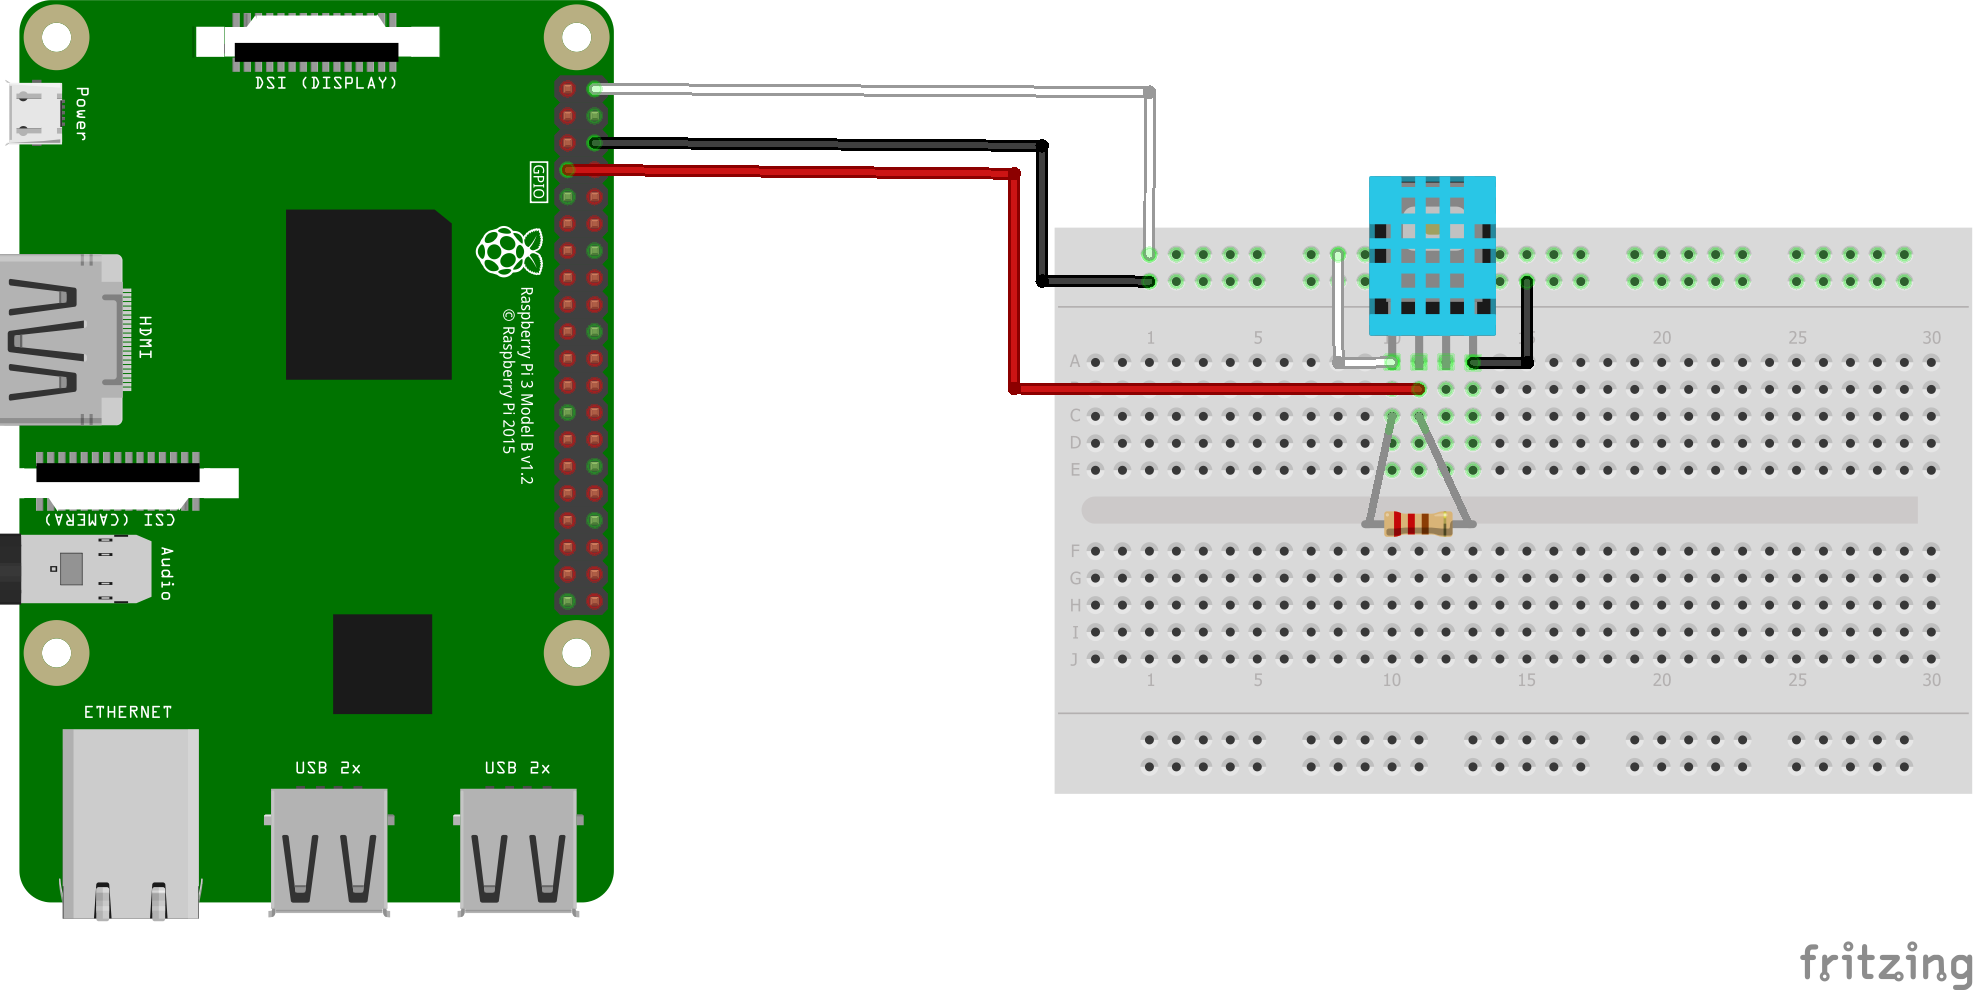
\includegraphics[height=2.5in]{figures/nodo_1.png}
\end{figure}

Clonamos la libreria del sensor, nos ubicamos en la ruta descargada \path{cd Adafruit_Python_DHT} e instalamos la libreria 'sudo python setup.py install', previamente instalamos las dependencias del la libreria para su instalacion 'sudo apt-get install python-setuptools' considerando que tenemos la version de python 2.7.3, esto permitira instalar la libreria de python para el sensor DHT version 1.4
